% \documentclass{jlreq}
\documentclass[xelatex,ja=standard,jafont=noto]{bxjsarticle}

%%============================
%====  PACKAGE IMPORT    ====
%%=========================
\usepackage{hyperref}
\usepackage[svgnames]{xcolor} % Enabling mixing colors and color's call by 'svgnames'
\usepackage{url} %URLをbibtexで表示する
\usepackage{fancyhdr}
\usepackage{graphicx}
\graphicspath{ {./img/} }

%%============================
%====  HEADER / FOOTER   ====
%%=========================
\pagestyle{fancy} %pagestyleはお好みで
%% Top
    \lhead{Teacher\ Name} %L
    % \chead{Center} %C
    \rhead{Class\ Name} %R
%% Bottom
    % \lfoot{フッタ左} %L
    \cfoot{—\, \thepage \, —} %C.ページ番号を表示
    % \rfoot{© 著作権} %R

%%============================
%====   Code Settings    ====
%%=========================
\usepackage{listings,jvlisting} 
%日本語のコメントアウトをする場合jvlisting(もしくはjlisting)が必要
%ここからソースコードの表示に関する設定
\lstset{
  basicstyle={\ttfamily},
  identifierstyle={\small},
  commentstyle={\smallitshape},
  keywordstyle={\small\bfseries},
  ndkeywordstyle={\small},
  stringstyle={\small\ttfamily},
  frame={tb},
  breaklines=true,
  columns=[l]{fullflexible},
  numbers=left,
  xrightmargin=2 cm,
  xleftmargin=2 cm,
  numberstyle={\scriptsize},
  stepnumber=1,
  numbersep=0.2 cm,
  lineskip=-0.5ex
}
\renewcommand{\lstlistingname}{コードブロックのタイトル}

%%============================
%==  COLOR & FONT SETTING  ==
%%=========================
\definecolor{MyColor1}{rgb}{0.4,0.4,0.5} %mix personal color
\newcommand{\blueb}{\color{MyColor1}\usefont{OT1}{NotoSansCJKjp-Black}{b}{n}}
% \newcommand{\blueb}{\color{MyColor1} \usefont{OT1}{lmss}{b}{n}}

%%============================
%========  bibTeX   =========
%%=========================
% \usepackage[
% backend=biber,
% style=alphabetic,
% sorting=ynt
% ]{biblatex}
% \addbibresource{ref.bib}
%\renewcommand{\refname}{XXXXXXXX}
\renewcommand{\bibname}{\centering{参考文献}}%中央よせ

%%============================
%======  Font Weight  =======
%%=========================
% 使用するウェイトを変更する場合
%\documentclass[xelatex,ja=standard]{bxjsarticle}
%\setCJKmainfont[BoldFont=NotoSerifCJKjp-Black]{NotoSerifCJKjp-Light}
% \setCJKsansfont[BoldFont=NotoSansCJKjp-Black]{NotoSansCJKjp-Light}
%\setCJKmonofont[BoldFont=NotoSansCJKjp-Black]{NotoSansCJKjp-Light}

%%============================
%======    ESCAPE     =======
%%=========================
% 和文扱いにしたい文字の個別登録
\xeCJKDeclareCharClass{CJK}{`①,`⑵,`Ⅲ,`☃} 

%%============================
%======      NOTE     =======
%%=========================
% \gtfamily : ゴシック体
% \mdseries : 普通の太さの文字
% \upshape : 普通の形の文字

%% BEGIN TITLE HEAD   ==================================
\title{\blueb\gtfamily\mdseries\upshape\rmfamily\textsf{The Awesome Title \& Noto Sans CJK Template\\ \Large For Japanese Class Assignment}}
\author{\gtfamily 村上貴人
\thanks{筑波大学, 情報学群, 知識情報・図書館学類 (Univ. of Tsukuba)} 
\thanks{国立研究開発法人 産業技術総合研究所 (AIST),  メディアインタラクション研究グループ} 
\thanks{takahito[at]digitalnature.slis.tsukuba.ac.jp} } 
%名前とかは\footnote{}より\thanks{}を使った方がいいっぽい

\date{\textsf{Jul. 6, 2021}}
%% BEGIN BODY  =========================================
\begin{document}
\maketitle
\thispagestyle{fancy} %% 1ページ目にヘッダーが必要な場合
% \newpage タイトルで改ページをする場合
\ \\\\
\section{Usage}
このテンプレートは授業レポート用に先人のテンプレートを改良したものです。Overleaf上でXeLa\TeX で使うために作られました。
基本的な使いかたは他の\TeX テンプレートと同じかと思います。
このテンプレートでは,Wordでのレポート作成に疲れたので,
\begin{itemize}
    \item 綺麗な色付きのタイトルが作れたり,
    \item Noto Sans/Serif CJKの美しい和文フォントが標準で使えたり,
\end{itemize}
などができます。また,\verb+ Noto Sans CJK+は\verb+\documentclass[xelatex,ja=standard,jafont=noto]{bxjsarticle}+でクラスレベルで読み込まれるので脳死で書くかことができます。\footnote{細かいことは気にしないんや。}
もし\TeX に逆に疲れたらWordなりPagesを使ったら良いと思います。


その他は\TeX と変わらないと思います。例を挙げると,\\
\textrm{Roman\ デフォルト} \\
\textgt{Gothic\ 和文ゴシック体} \\
\textbf{Boldface\ 太字} \\
\textit{Italic\ 斜体} \\
\textsl{Slanted\ ローマンを傾けただけ} \\
\textsf{Sans Serif\ サンセリフ体} \\
\texttt{Typewriter\ タイプライタ体、等幅} \\
\textsc{Small Caps\ 小文字が大文字に} \\

\section{Section}
\subsection{Sub Section}
\subsection{Sub Sub Section}

等があります。図を挿入してセンタリングはときは,
\begin{figure}[h] %hを入れないと改行して挿入したことにならない
    \centering
    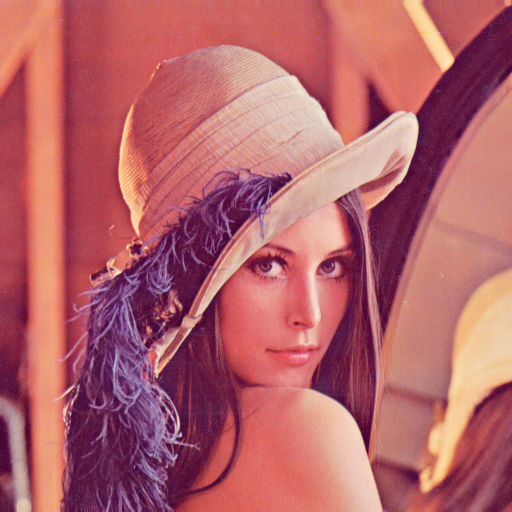
\includegraphics[scale=0.3]{lena}
    \caption{有名なlena}
    \label{lena}
\end{figure}

でできます。2つ並べるには(図 \ref{miro1})。

\begin{figure}[h]
    \begin{tabular}{cc}
      %---- 最初の図 ---------------------------
      \begin{minipage}[t]{0.5\hsize}
        \centering
        
\includegraphics[width=0.8\textwidth]{1}
        \caption{左}
        \label{miro1}
      \end{minipage} &
      %---- 2番目の図 --------------------------
      \begin{minipage}[t]{0.5\hsize}
        \centering
        
\includegraphics[width=0.8\textwidth]{2}
        \caption{右}
        \label{miro2}
      \end{minipage}
      %---- 図はここまで ----------------------
    \end{tabular}
\end{figure}

\newpage

参考文献は自動挿入されるのでbib\TeX を使います\footnote{コードは\url{https://qiita.com/ta_b0_/items/2619d5927492edbb5b03}}。
\begin{lstlisting}[caption=bib\TeX]
\nocite{*}
\bibliography{ref.bib}
\bibliographystyle{plain}
\end{lstlisting}
この順番を守らないといけないらしい。


\verb+\nocite{*}+を使うと使われてない参考文献も全部でる。

\nocite{*}
\bibliography{ref.bib}
\bibliographystyle{plain}

\end{document}
